\documentclass[11pt]{article}

% --- Packages ---
\usepackage{graphicx}   % figures
\usepackage{float}      % better figure placement
\usepackage{dblfloatfix} % supports figure* in 2-column layouts (safe to include)

\usepackage{amsmath, amssymb} % optional but standard for reports
\usepackage{adjustbox}
\usepackage{placeins}

\begin{document}


\section*{Appendix 1: attributes}
\label{app1}

Detailed list of attributes used in the ablation study (all attributes combined are used for all other experiments):
\begin{itemize}
\item baseline: 
\begin{itemize}
\item to\_move: which side moves first
\item cp\_eval: Stockfish's centipawn evaluation of the initial position
\item moveXcp: Stockfish's centipawn evaluation of the position after X moves have been made (only best move is considered at each turn).
\item nodes:
\item selective depth: number of half-moves calculated by the engine in the most forcing variation.
\item WDL: win/draw/loss probability reported by the engine
\end{itemize}
\item counts: total material count for each player, counts for each piece for each player (e.g. number of white queens on the board). 
\item study:
\begin{itemize}
\item number of meaningful moves at level L: an attempt to count the number of moves human players would consider meaningful in the given position.
\item branching at level L: branching factor that takes into account only meaningful moves. 
\item average branching: an average of branching factors over all layers.
\item narrow solution at level L: counts the number of "forced" moves (that is, positions in which only one move leads to a good position). 
\item distance at level L: length between starting and target square for each move (that is, actual number of squares between the two squares).
\item pieces at level L: number of different pieces that move at level L.
\item all pieces involved: number of different pieces that move in the meaningful subtree. 
\item winning without checkmate: number of moves evaluated as winning that do not directly lead to a checkmate.
\item possible moves at level L: total number of legal moves at level L.
\item all possible moves: total number of legal moves at all levels.
\item all narrow solutions: sum of narrow solutions over all levels.
\item tree size: number of nodes in the meaningful search tree.
\item move ratio at level L: ratio between meaningful moves and possible moves. 
\item sum of distances over all levels.
\item average distance over all levels. 
\end{itemize}
\item Stockfish: engines with various strength settings (between 1320 and 3000) are used to evaluate the position. If their solution is aligned with the ground truth solution in the dataset, these attributes are given value 1, otherwise 0.
\item themes: 63 theme indicators provided in the original Lichess dataset. These include, for instance, "advancedPawn", "discoveredCheck", "doubleBishopMate", "mateIn4", "trappedPiece", etc. For each position, multiple themes can be present - for those, the attribute value is 1, otherwise 0.  
\end{itemize}













\clearpage

\section*{Appendix 2: Misclassifications}

In this part we inspect the most wrongly classified puzzles. We also inspected these specific samples with local SHAP 
explainer, where red arrows to right mean why model pushed classification towards classified class. Blue arrows to left 
mean that attribute contributed towards other classes. Besides the attributes there is also it's value. 

\vspace{10pt}
In the following figures \ref{6k1/r1b1q3/2p3p1/2Pp4/1P2p1n1/2B1P3/NQ6/2K4R w - - 0 1} \ref{rn3rk1/p5pp/3N4/4np1q/5Q2/1P6/PB1P1KP1/2R4R b - - 0 1} 
\ref{8/p1p1k2p/4P3/2PP1p1P/1r3r2/5B2/P3RK2/8 w - - 0 1}
we show three examples where a model classified one puzzle as hard, although by 
lichess rating (ground truth) it is classified as easy. Besides the puzzle we also show the corresponding local SHAP explanator.

\vspace{5pt}
\noindent
We can see that there are a few attributes common in all three puzzles: 
\textit{long = 1}, \textit{short = 0}, \textit{solved1320 = 0}. It seems that the model 
taught itself that with that combination, the puzzle is more or less classified as easy.



\begin{figure}[!ht]
    \centering

    \begin{minipage}[t]{0.47\columnwidth}
        \centering
        \adjustbox{frame,center}{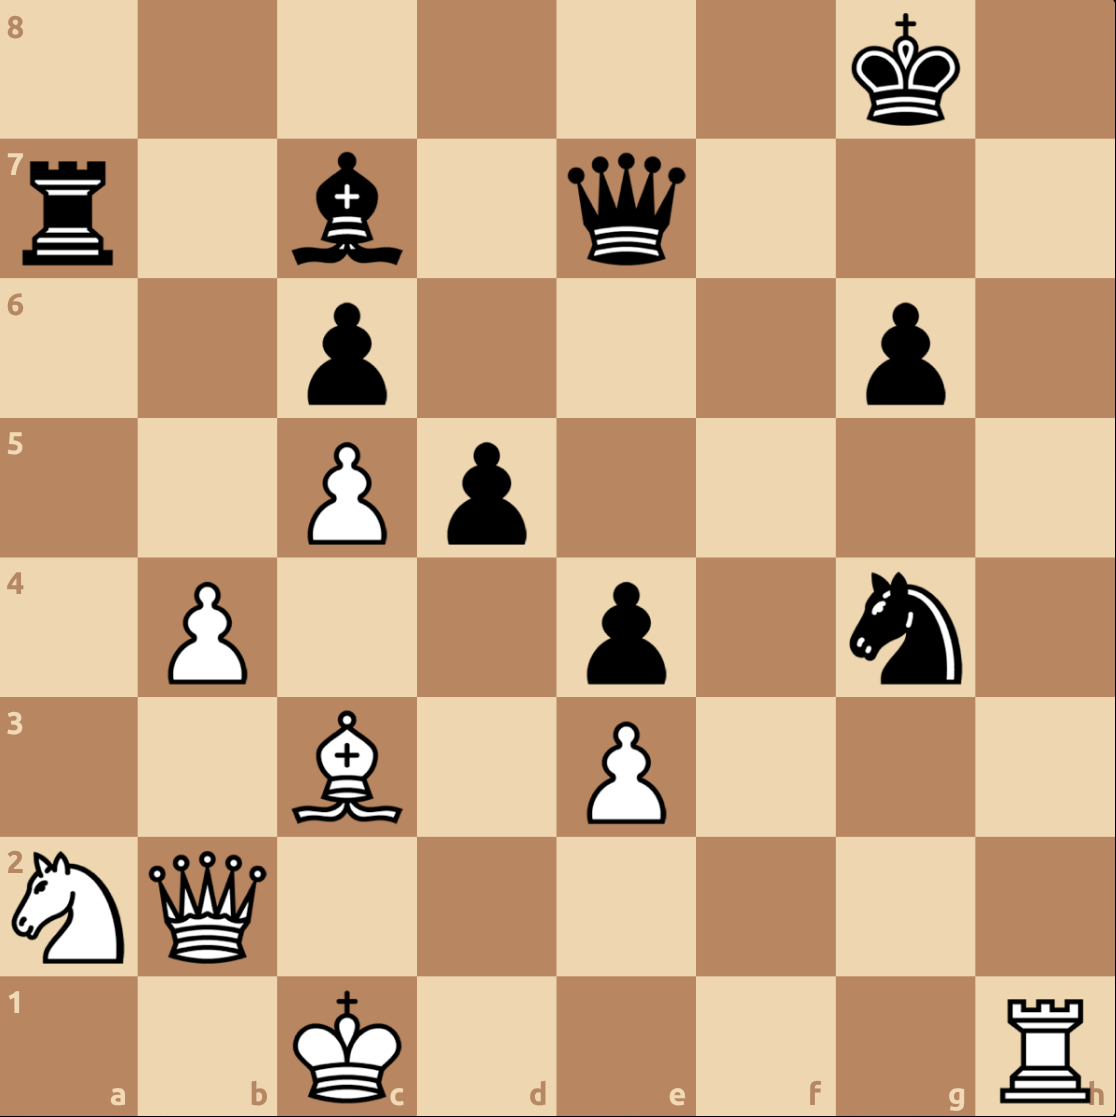
\includegraphics[height=5cm]{easy_puzzle_miss_1.png}}
        \caption{True label easy, classified as hard. White to move - solution: 1.Rh8+ Kf7 2. Rh7+ Ke8 3.Txe7}
        \label{6k1/r1b1q3/2p3p1/2Pp4/1P2p1n1/2B1P3/NQ6/2K4R w - - 0 1}
    \end{minipage}%
    \hfill
    \begin{minipage}[t]{0.47\columnwidth}
        \centering
        \adjustbox{frame,center}{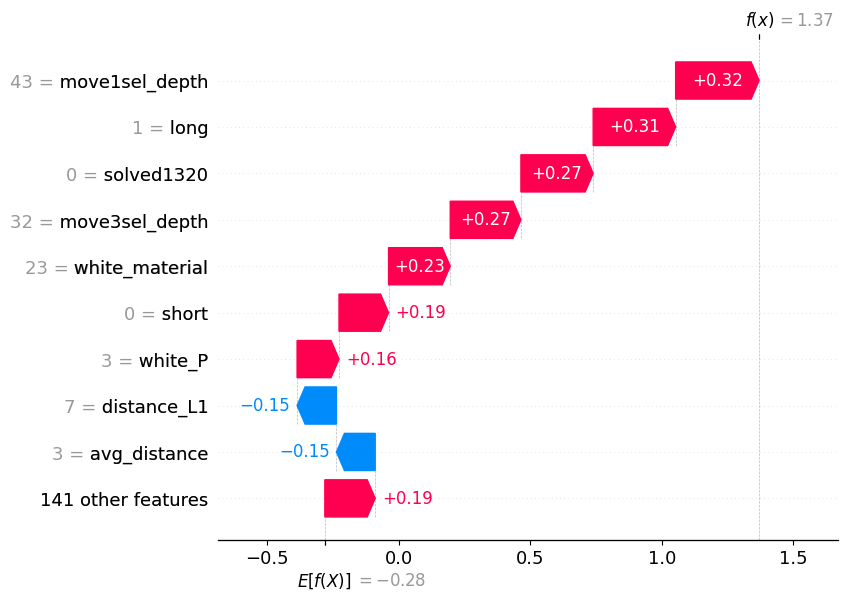
\includegraphics[height=5cm]{easy_puzzle_miss_1_shap.png}}
        \caption{Shap for Figure \ref{6k1/r1b1q3/2p3p1/2Pp4/1P2p1n1/2B1P3/NQ6/2K4R w - - 0 1}}
        \label{shap 6k1/r1b1q3/2p3p1/2Pp4/1P2p1n1/2B1P3/NQ6/2K4R w - - 0 1}
    \end{minipage}%

\end{figure}
\FloatBarrier



\begin{figure}[!ht]
    \centering

    \begin{minipage}[t]{0.47\columnwidth}
        \centering
        \adjustbox{frame,center}{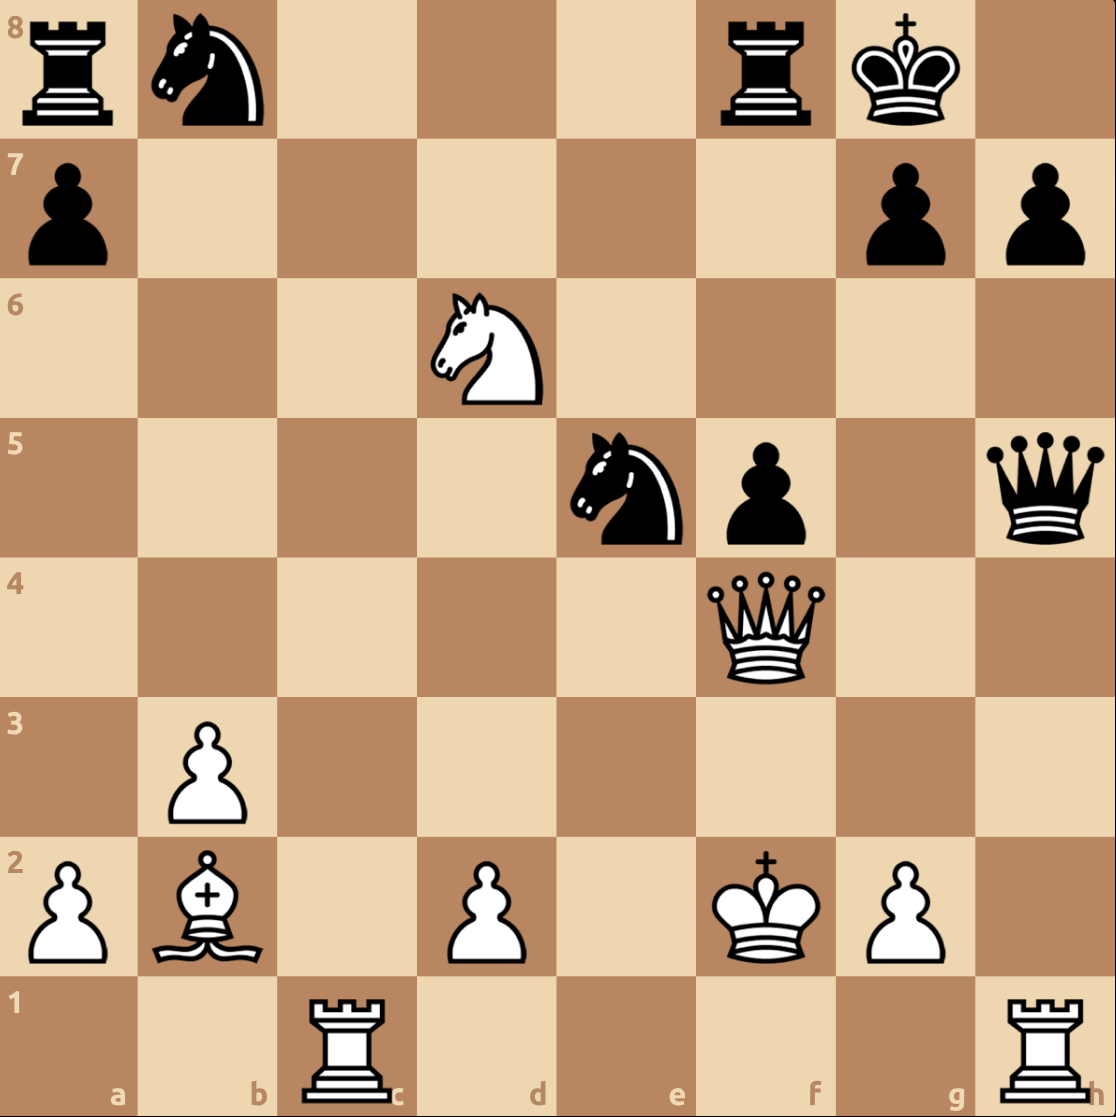
\includegraphics[height=5cm]{easy_puzzle_miss_2.png}}
        \caption{True label easy, classified as hard. Black to move - solution: 1...Sd3+ 2.Ke3 Sxf4 3.Txh5 Sxh5}
        \label{rn3rk1/p5pp/3N4/4np1q/5Q2/1P6/PB1P1KP1/2R4R b - - 0 1}
    \end{minipage}%
    \hfill
    \begin{minipage}[t]{0.47\columnwidth}
        \centering
        \adjustbox{frame,center}{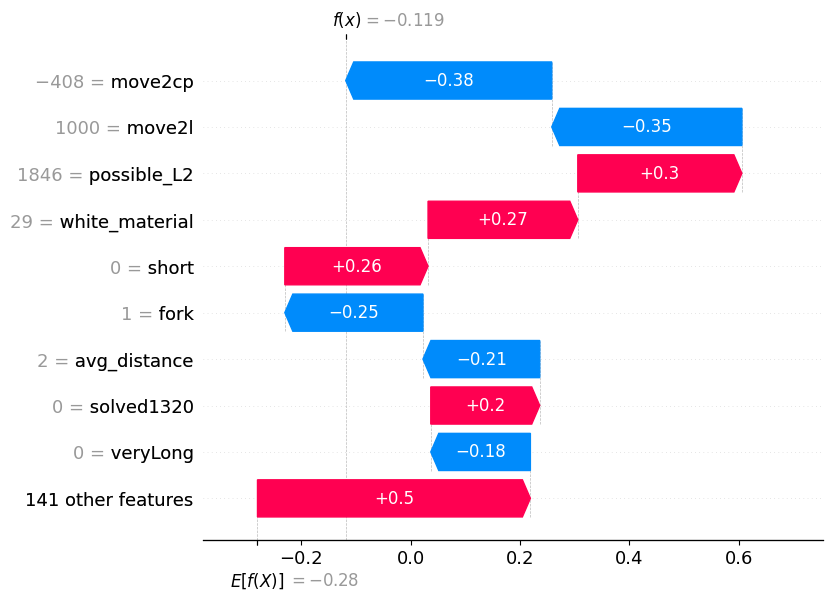
\includegraphics[height=5cm]{easy_puzzle_miss_2_shap.png}}
        \caption{Shap for Figure \ref{rn3rk1/p5pp/3N4/4np1q/5Q2/1P6/PB1P1KP1/2R4R b - - 0 1}}
        \label{shap rn3rk1/p5pp/3N4/4np1q/5Q2/1P6/PB1P1KP1/2R4R b - - 0 1}
    \end{minipage}%

\end{figure}
\FloatBarrier




\begin{figure}[!ht]
    \centering

    \begin{minipage}[t]{0.47\columnwidth}
        \centering
        \adjustbox{frame,center}{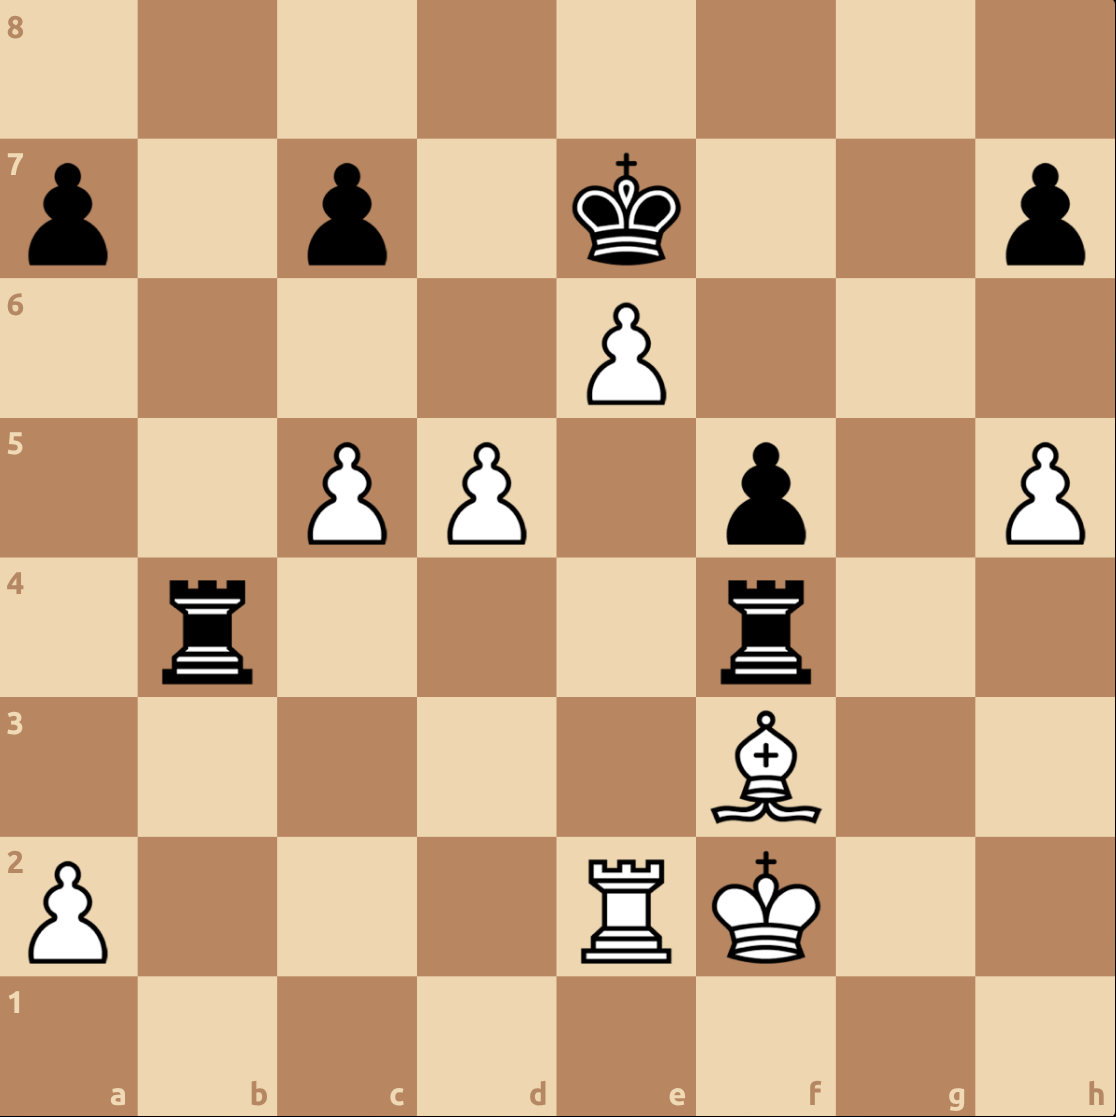
\includegraphics[height=5cm]{easy_puzzle_miss_3.png}}
        \caption{True label easy, classified as hard. White to move - solution: 1.d6+ exd6 2.exd6+ Kxd6 3.e7}
        \label{8/p1p1k2p/4P3/2PP1p1P/1r3r2/5B2/P3RK2/8 w - - 0 1}
    \end{minipage}%
    \hfill
    \begin{minipage}[t]{0.47\columnwidth}
        \centering
        \adjustbox{frame,center}{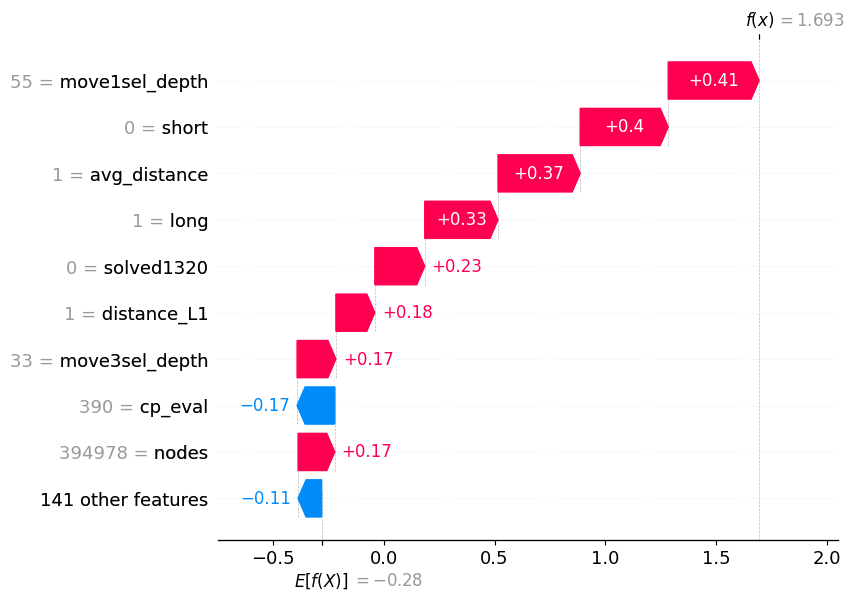
\includegraphics[height=5cm]{easy_puzzle_miss_3_shap.png}}
        \caption{Shap for Figure \ref{8/p1p1k2p/4P3/2PP1p1P/1r3r2/5B2/P3RK2/8 w - - 0 1}}
        \label{shap 8/p1p1k2p/4P3/2PP1p1P/1r3r2/5B2/P3RK2/8 w - - 0 1}
    \end{minipage}%

\end{figure}
\FloatBarrier




%%%%%%%%%%%%%%%%%%%%%%%%%%%%%%%%%%%%%%%%%%%%%%%%%%%%%%%%%%%%%%%%%%%%%%%%%%%%%%%%%%%%%%%%%%%%%%%
\clearpage

In the following figures \ref{r3k3/ppp2p2/1b1p3p/4p2r/2B1P1bq/P1PP1P2/1P4PQ/RN3R1K w q - 0 1},
\ref{4Rrk1/p6p/1pp2rp1/8/5B1q/4QP1P/P1P2PK1/8 w - - 0 1}, \ref{4rrk1/ppp2pp1/7p/3n4/3P3q/1P2p2P/PB4P1/R2QRBK1 b - - 0 1}
we also show the opposite big misclassification - puzzle rating (ground truth)
is hard, while the model predicted it as easy. 

\vspace{5pt}
\noindent
Here we can see that the opposite attributes contribute the most to that classification: 
\textit{short = 1}, \textit{long = 0}, and \textit{solved1320 = 1}. There is one another attribute 
that contributes a lot towards the lower rating classification, \textit{fork = 1}.

\vspace{5pt}
\noindent
Another thing that a chess player might notice is the ground truth label of these puzzles. 
Subjectively speaking, the model might have created a better label than the real label of 
the puzzle. On the first sight some the puzzles are not that hard - we could easily put them 
in a lower rated categories. 



\begin{figure}[!ht]
    \centering

    \begin{minipage}[t]{0.47\columnwidth}
        \centering
        \adjustbox{frame,center}{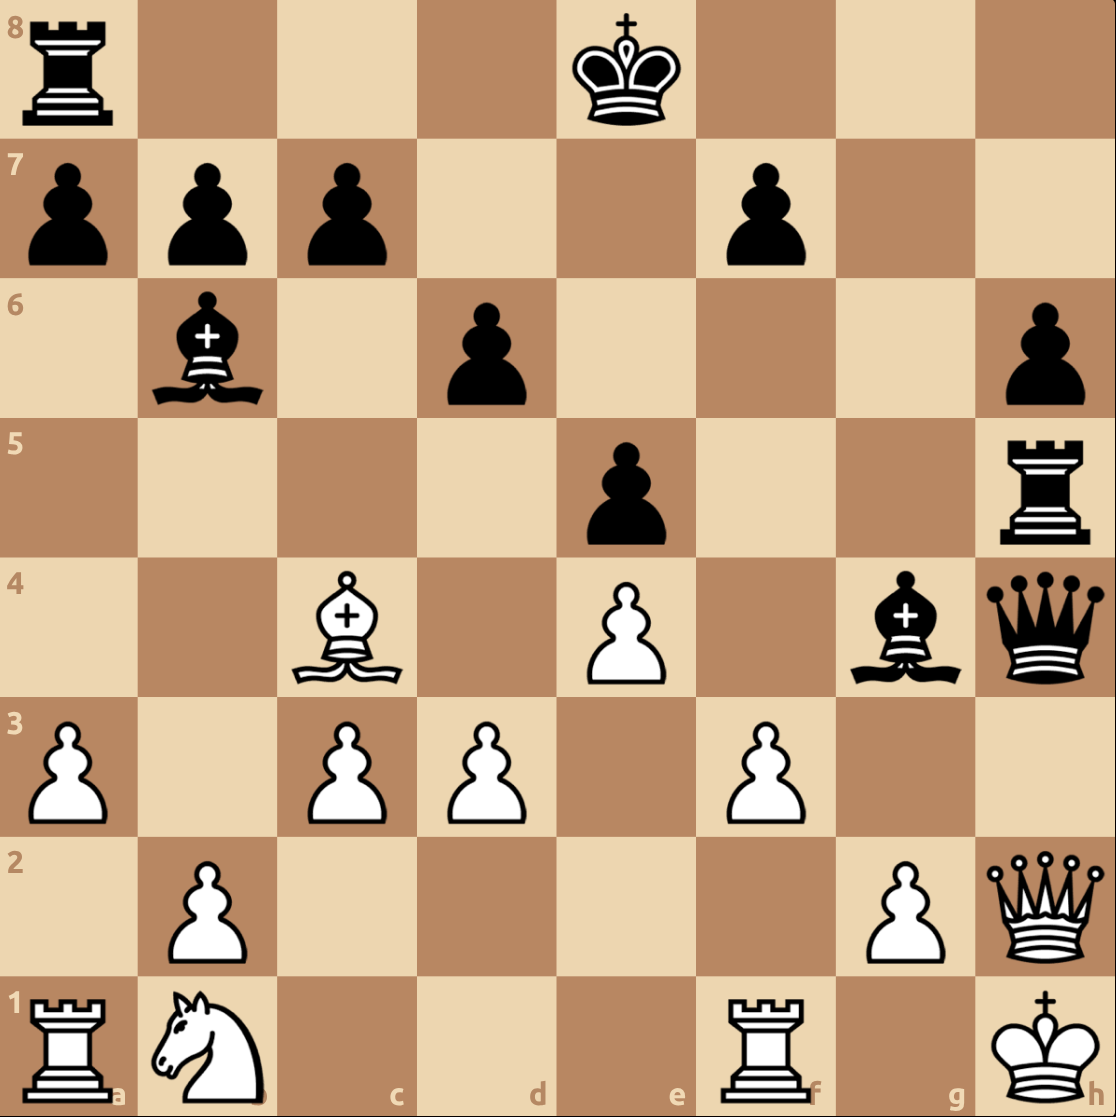
\includegraphics[height=5cm]{hard_puzzle_miss_1.png}}
        \caption{True label hard, classified as easy. White to move - solution: 1.Bxf7+ Ke7 2.Bxh5}
        \label{r3k3/ppp2p2/1b1p3p/4p2r/2B1P1bq/P1PP1P2/1P4PQ/RN3R1K w q - 0 1}
    \end{minipage}%
    \hfill
    \begin{minipage}[t]{0.47\columnwidth}
        \centering
        \adjustbox{frame,center}{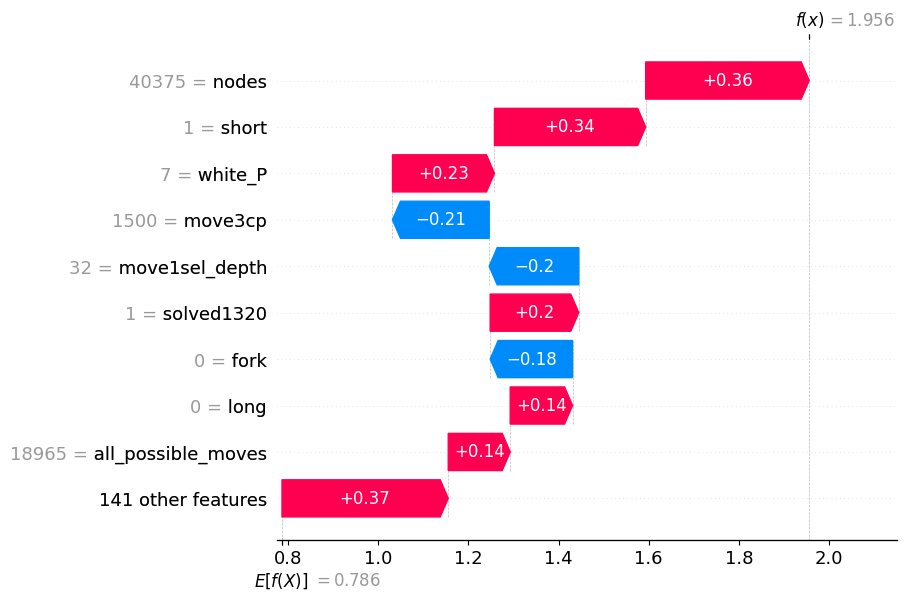
\includegraphics[height=5cm]{hard_puzzle_miss_1_shap.png}}
        \caption{Shap for Figure \ref{r3k3/ppp2p2/1b1p3p/4p2r/2B1P1bq/P1PP1P2/1P4PQ/RN3R1K w q - 0 1}}
        \label{shap r3k3/ppp2p2/1b1p3p/4p2r/2B1P1bq/P1PP1P2/1P4PQ/RN3R1K w q - 0 1}
    \end{minipage}%

\end{figure}
\FloatBarrier



\begin{figure}[!ht]
    \centering

    \begin{minipage}[t]{0.47\columnwidth}
        \centering
        \adjustbox{frame,center}{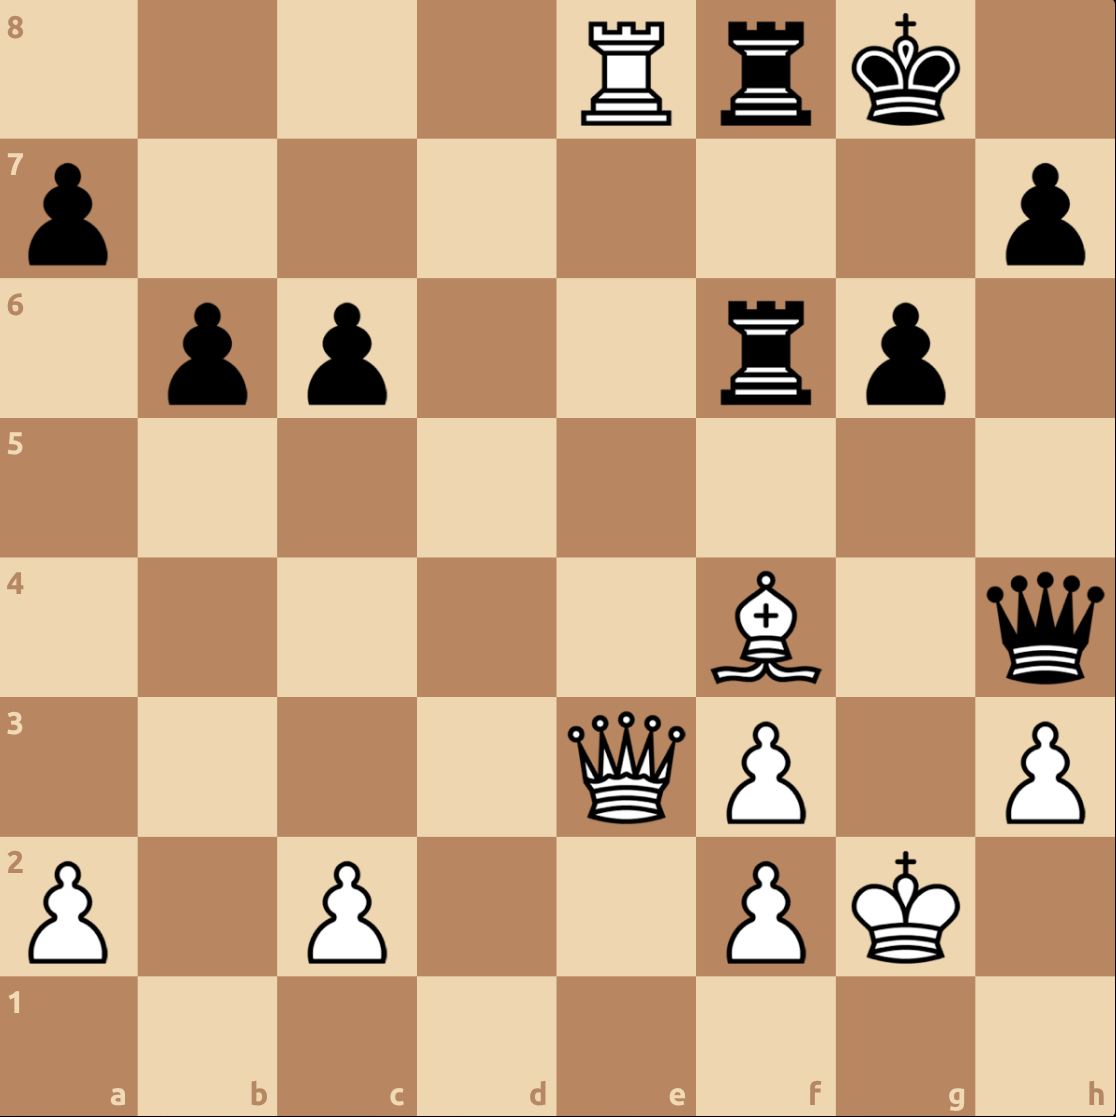
\includegraphics[height=5cm]{hard_puzzle_miss_2.png}}
        \caption{True label hard, classified as easy. White to move - solution: 1.Bg5 Qxg5 2.Qxg5}
        \label{4Rrk1/p6p/1pp2rp1/8/5B1q/4QP1P/P1P2PK1/8 w - - 0 1}
    \end{minipage}%
    \hfill
    \begin{minipage}[t]{0.47\columnwidth}
        \centering
        \adjustbox{frame,center}{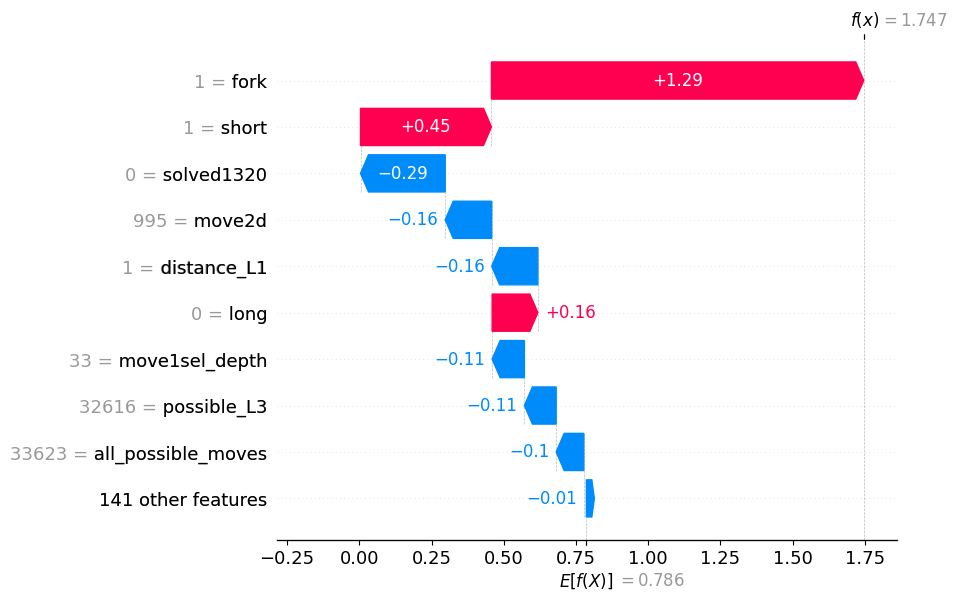
\includegraphics[height=5cm]{hard_puzzle_miss_2_shap.png}}
        \caption{Shap for Figure \ref{4Rrk1/p6p/1pp2rp1/8/5B1q/4QP1P/P1P2PK1/8 w - - 0 1}}
        \label{shap 4Rrk1/p6p/1pp2rp1/8/5B1q/4QP1P/P1P2PK1/8 w - - 0 1}
    \end{minipage}%

\end{figure}
\FloatBarrier




\begin{figure}[!ht]
    \centering

    \begin{minipage}[t]{0.47\columnwidth}
        \centering
        \adjustbox{frame,center}{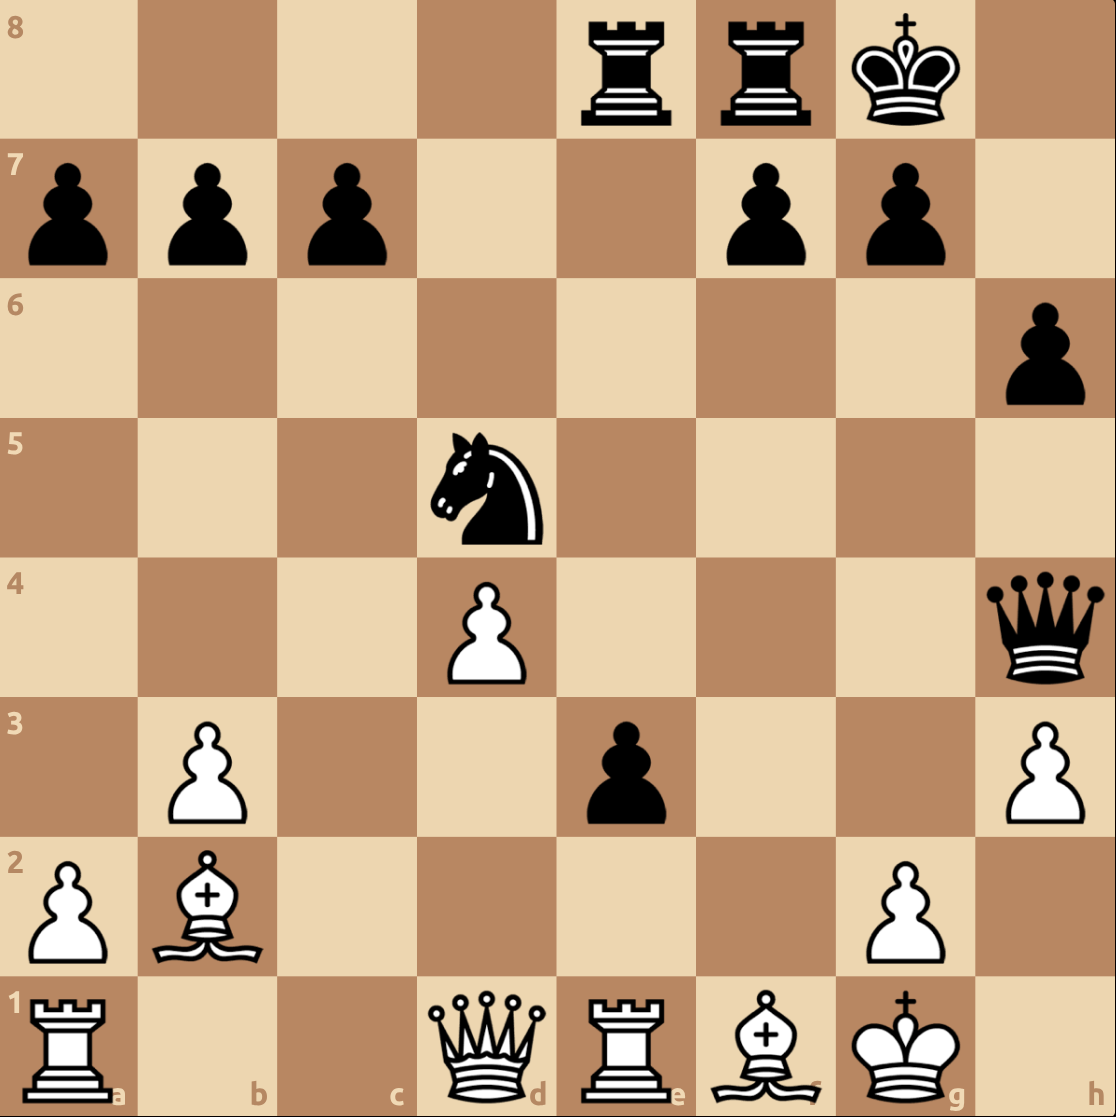
\includegraphics[height=5cm]{hard_puzzle_miss_3.png}}
        \caption{True label hard, classified as easy. Black to move - solution: 1...Qf2+ 2.Kh2 Qxb2}
        \label{4rrk1/ppp2pp1/7p/3n4/3P3q/1P2p2P/PB4P1/R2QRBK1 b - - 0 1}
    \end{minipage}%
    \hfill
    \begin{minipage}[t]{0.47\columnwidth}
        \centering
        \adjustbox{frame,center}{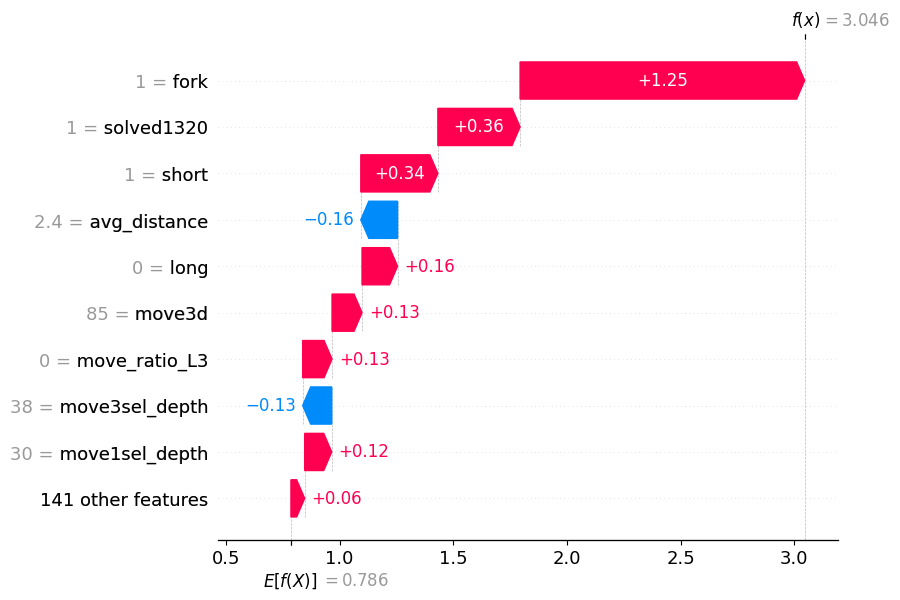
\includegraphics[height=5cm]{hard_puzzle_miss_3_shap.png}}
        \caption{Shap for Figure \ref{4rrk1/ppp2pp1/7p/3n4/3P3q/1P2p2P/PB4P1/R2QRBK1 b - - 0 1}}
        \label{shap 4rrk1/ppp2pp1/7p/3n4/3P3q/1P2p2P/PB4P1/R2QRBK1 b - - 0 1}
    \end{minipage}%

\end{figure}
\FloatBarrier





\clearpage

\section*{Appendix 3: Interpretability}

To explain how to model makes decisions, we used SHAP global explainer. We used it on XGBoost model. 
Figure \ref{inter} shows the beeswarm plot of the top attributes. One dot means one sample from the test 
set. Blue dot means this sample has small value of that attribue, red means high. If a dot is more on the 
left side, it means that that attribute contributed towards lower rating classification, while on the right 
side towards higher rating classification.

\vspace{5pt}
We can see a few very distinct attributes (by that we mean the ones where most of the blue dots are on one side,  
and most of the red dost are on the other side). Here we explain few of them:

\begin{itemize}
    \item \textit{move1sel\_depth}: If a forced line is short (blue dot), then rating will be lower. This intuitively makes sense since a less strong player is also likely to find a short forced line.
    \item \textit{solved1320}: If Stockfish engine with strength 1320 was able to solve that puzzle (red dot), then the predicted rating will be lower. That also makes sense, however, it is interesting enough that only one of the engine strenghts is in top 10 attributes.
    \item \textit{short}, \textit{long}, \textit{veryLong}: very similar logic as for \textit{move1sel\_depth}. Shorter puzzles lead to lower rating predictions, which is sensible because lower rated players are on average more likely to successfully solve short puzzles than long ones.
    \item \textit{fork}: another intuitively logical outcome - if a puzzle includes forks, it is classified as easier one. Subjectively speaking, forks are usually one of the easiest motifs to see.
\end{itemize}


 

\begin{figure*}[!htbp]
    \centering
    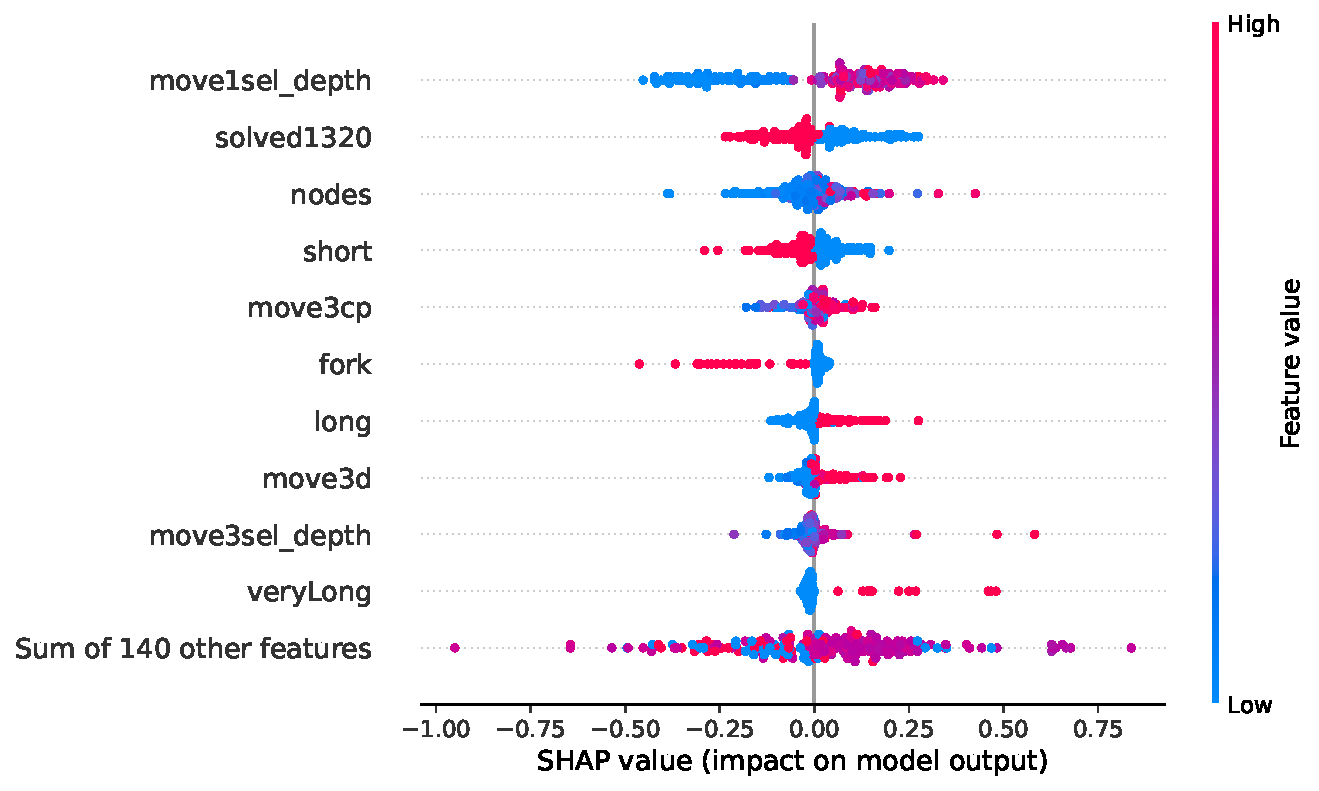
\includegraphics[width=1\textwidth]{shap.pdf}
    \caption{SHAP values for XGBoost Classifier}
    \label{inter}
\end{figure*}
\FloatBarrier

Intuitively, the model does make logical decisions. However, it seems that chess might be too hard to 
predict it's difficulty for people just from the gathered attributes. 




\end{document}